%%%%%%%%%%%%%%%%%%%%%%%%%%%%%%%%%%%%
%%%%  Author: Aakash Ravichandran %%%%
%%%%  Description: Discrete Fourier Transform, FFT analysis, spectral leakage effects
%%%%%%%%%%%%%%%%%%%%%%%%%%%%%%%%%%%%

\documentclass[../main]{subfiles}
\begin{document}

\chapter{Signal Analysis}
\label{cha:signal_analysis}

Signal analysis is performed in this chapter. The aim is to first provide a brief introduction
to the Discrete Fourier Transform (DFT) in the context of its application to multi-frequency analysis
for flutter derivative identification. This is then applied to single- and multi-frequency signal extraction.
Finally, potential sources of error and methods to mitigate them are discussed.\\

The Fourier Transform is a mathematical tool used to convert a signal from the time domain to
the frequency domain. Since real-world data consists of discrete numbers rather than continuous
mathematical functions, the transform cannot be applied directly. Therefore, the Discrete
Fourier Transform (DFT) is used in such cases. The DFT converts time-varying data into the
frequency domain, and its inputs are the time-varying data and the sampling frequency. The
sampling frequency defines how many samples are taken per second; in the CFD context,
it is equal to $1/\Delta t$, where $\Delta t$ is the time step.\\

The Fast Fourier Transform (FFT) is derived from the DFT, which has significantly higher
computational efficiency. Several open-source tools are available to perform FFT computations,
one of which is provided by the \texttt{scipy.fft} module in Python \cite{scipy}. Since Python is used for
post-processing throughout this thesis, the SciPy FFT tool is used to convert the obtained
aerodynamic forces and moments into the frequency domain.\\

Since the DFT operates on a discrete set of values, it is subject to certain inherent
limitations that can affect the quality of the transformation and the usability of its results.
It is therefore necessary to study these issues before applying the FFT to flutter derivative
calculations. This is the focus of the present chapter: to examine the issues associated with
the DFT and to investigate its efficient application in the multi-frequency method for flutter
derivative identification.\\

The accuracy of extracting the amplitude of a particular signal using the FFT depends on two
parameters:

\begin{enumerate}
    \setlength{\itemsep}{0pt}\setlength{\parskip}{0pt}
    \item The frequency of the signal to be extracted.
    \item The frequency bin of the data.
\end{enumerate}

The frequency bin refers to the discrete set of frequency values produced by the FFT during
domain conversion. If the frequency of the signal to be extracted coincides with one of the
values in the frequency bin, the extracted amplitude will be accurate and free from
discretisation errors. If the signal frequency does not coincide with a frequency bin value, the amplitude obtained
from the FFT will contain an error. This effect is known as spectral leakage: This happens because since 
no bin directly corresponds to the signal frequency, its amplitude is distributed across the
neighbouring bins. The frequency bins of a time data is calculated as

\begin{equation}
f_k = k \cdot \frac{f_s}{N}, \qquad k = 0, 1, 2, \dots, \left\lfloor \frac{N}{2} \right\rfloor
\end{equation}

where
\begin{itemize}
    \item $f_k$ \quad = frequency of the $k$-th frequency bin (Hz)
    \item $k$     \quad = frequency bin index 
    \item $f_s$   \quad = sampling frequency (Hz)
    \item $N$     \quad = length of the data
    \item $\Delta f = \frac{f_s}{N}$ \quad = frequency resolution / bin width (Hz)
\end{itemize}

\vspace{0.3cm}

The spacing between two adjacent frequencies in the bin is known as the bin spacing,
and the frequency resolution of an FFT refers to how small this spacing is. A smaller
bin spacing corresponds to a higher frequency resolution. As shown by the formula, the
resolution depends on the length of the data record.\\

Another important issue to be aware of is aliasing. The maximum signal frequency that
can be extracted using an FFT is limited by the Nyquist frequency, given by:

\begin{equation}
    f_{\text{Nyquist}} = \frac{f_s}{2}
\end{equation}

where $f_s$ is the sampling frequency. This can create issues in two ways. First, if
the frequency of interest lies above the Nyquist frequency, it cannot be extracted. Second,
even if the frequency of interest lies within the Nyquist limit, any other signal with a
frequency above it will be folded back into the valid frequency range by the FFT. If such a
folded component does not fall on a bin, it will introduce additional spectral leakage. While
the probability of this occurrence is
low, this effect should be kept in mind when using the FFT in practice.\\

These two effects combined impose restrictions on the frequencies that can be extracted and
the accuracy with which they can be obtained, in various forms. These are studied for 
single- and multi-frequency methods in the following sections. \\

% \begin{enumerate}
%     \item As discussed, if the frequency of interest does not have a finite decimal
%           representation or does not fall on a frequency bin, spectral leakage will introduce
%           error.
%     \item The length of the data record determines a frequency bin that may or may not match
%           the frequency of interest.
%     \item The frequency of interest must lie within the Nyquist frequency.
%     \item If random noise such as white noise is present in the data, the extracted amplitude
%           will contain error even if the signal frequency falls on a bin. This is because random
%           noise excites many frequencies simultaneously, and any overlap with the frequency range
%           of the signal of interest will disturb the extracted amplitude. Since the noise is
%           random, a large bin spacing further compounds this error through spectral leakage.
% \end{enumerate}

% ============================================================
\section{Single Frequency}
% ============================================================

This section studies the effects discussed in Section~1 as applied to a single-frequency
signal. A sample sine wave is generated with discrete points, passed to the FFT tool from the
SciPy module, and the resulting amplitudes are analyzed. Since the amplitude of the input
signal is known, it is compared against the FFT output and the error is examined for the
following cases:

\begin{enumerate}
    \setlength{\itemsep}{0pt}\setlength{\parskip}{0pt}
    \item Bin Match
    \item Non-Bin Match
    \item Bin Match with Noise
    \item Frequency Bin Resolution on Non-Matching Bin
\end{enumerate}

Throughout this section, the input signal has a total duration of 10 seconds and is sampled at a frequency of 500~Hz. 
With these parameters, the resulting frequency bins range from 0 to 250.0~Hz, with a bin spacing of 0.1~Hz 
(i.e., 0, 0.1, 0.2, 0.3, 0.4, 0.5, 0.6, \ldots, 250.0~Hz). The maximum frequency of 250~Hz corresponds to the Nyquist 
limit, which represents half the sampling frequency and is the highest frequency that can be accurately represented by 
the discrete sampling.

% ------------------------------------------------------------
\subsection{Bin Match}
% ------------------------------------------------------------

A signal with a frequency of 0.4~Hz and an amplitude of 1.0 is used as input. Since 0.4~Hz
falls directly on a frequency bin, no spectral leakage is expected. 
As shown in Figure~\ref{fig:sf_binmatch}, the amplitude output from the FFT is 1.00, which
matches the input signal amplitude exactly. This confirms that, when the signal frequency falls
on a frequency bin, no discretisation error is introduced. 

\begin{figure}[htbp]
    \centering
    \begin{subfigure}[b]{0.45\textwidth}
        \centering
        
\includegraphics[width=\textwidth]{Figures/SingleFrequency/1_Input_Signal.png}
        \caption{Signal}
        \label{fig:sf_binmatch_input}
    \end{subfigure}
    \hfill
    \begin{subfigure}[b]{0.45\textwidth}
        \centering
        
\includegraphics[width=\textwidth]{Figures/SingleFrequency/1_Spectrum.png}
        \caption{Amplitude spectrum}
        \label{fig:sf_binmatch_spectrum}
    \end{subfigure}
    
\caption{Single-frequency bin-match case: input signal and corresponding FFT spectrum.}
    \label{fig:sf_binmatch}
\end{figure}

% ------------------------------------------------------------
\subsection{Non-Bin Match}
% ------------------------------------------------------------

In this case, the input signal frequency is changed to 0.45~Hz, which does not coincide with
any frequency bin. Since 0.45~Hz lies midway between the 0.4~Hz and 0.5~Hz bins, the FFT
assigns its amplitude to the nearest neighbouring bin. \\

\begin{figure}[htbp]
    \centering
    \begin{subfigure}[b]{0.45\textwidth}
        \centering
        
\includegraphics[width=\textwidth]{Figures/SingleFrequency/2_Input_Signal.png}
        \caption{Signal}
        \label{fig:sf_nonbinmatch_input}
    \end{subfigure}
    \hfill
    \begin{subfigure}[b]{0.45\textwidth}
        \centering
        
\includegraphics[width=\textwidth]{Figures/SingleFrequency/2_Spectrum.png}
        \caption{Amplitude spectrum}
        \label{fig:sf_nonbinmatch_spectrum}
    \end{subfigure}
    
\caption{Single-frequency non-bin-match case: input signal and corresponding FFT spectrum showing spectral leakage.}
    \label{fig:sf_nonbinmatch}
\end{figure}

As shown in Figure~\ref{fig:sf_nonbinmatch}, the extracted amplitude is 0.653, corresponding
to an error of 34.70\%. This demonstrates that when the signal frequency does not fall on a
frequency bin, spectral leakage causes a significant reduction in accuracy.

% ------------------------------------------------------------
\subsection{Bin Match with Noise}
% ------------------------------------------------------------

In this case, the input signal is kept at 0.4~Hz. Additionally, white noise with an amplitude
of 0.2 is superposed on the signal to assess its effect on the extracted amplitude. 
As shown in Figure~\ref{fig:sf_noise}, the extracted amplitude is 0.99, corresponding to an
error of only 0.04\%. Although noise does introduce a small error, its effect is considerably
less severe than that of spectral leakage.

\begin{figure}[htbp]
    \centering
    \begin{subfigure}[b]{0.45\textwidth}
        \centering
        
\includegraphics[width=\textwidth]{Figures/SingleFrequency/3_Input_Signal.png}
        \caption{Signal}
        \label{fig:sf_noise_input}
    \end{subfigure}
    \hfill
    \begin{subfigure}[b]{0.45\textwidth}
        \centering
        
\includegraphics[width=\textwidth]{Figures/SingleFrequency/3_Spectrum.png}
        \caption{Amplitude spectrum}
        \label{fig:sf_noise_spectrum}
   
    \end{subfigure}
    \caption{Single-frequency bin-match case with added white noise: input signal and corresponding FFT spectrum.}
    \label{fig:sf_noise}
\end{figure}

% ------------------------------------------------------------
\subsection{Frequency Bin Resolution on Non-Matching Bin}
% ------------------------------------------------------------

The amplitude error associated with a non-bin-matched frequency is based on the relative
position of that frequency between its two nearest bins. The closer the frequency lies to the
midpoint between two adjacent bins, the greater the spectral leakage and, consequently, the
larger the resulting error.\\

To illustrate this, consider a signal at 0.54~Hz with the same configuration as above, where
the neighbouring frequency bins are located at 0.5~Hz and 0.6~Hz. This frequency falls near
the centre of the interval between the two adjacent bins, producing an error of 21.77\%. When
the total time is extended to 20~s, the bin spacing is reduced, placing the
neighbouring bins at 0.5~Hz and 0.55~Hz. In this finer-resolution case, the error decreases
to 5.6\%, since 0.54~Hz lies closer, in relative terms, to one of its neighbouring bins.\\

This behaviour is further illustrated by examining a signal at 0.53~Hz. In the first
configuration (bin spacing of 0.1~Hz), the normalised distance of 0.53~Hz from the midpoint
between its nearest bins is $0.3/0.5 = 0.6$, yielding an error of 11.68\%. In the second
configuration (bin spacing of 0.05~Hz), this ratio increases to $0.2/0.25 = 0.8$, and the
error rises to 24.02\%, despite the absolute distance to the nearest bin being smaller. This
result highlights that it is the relative position within the bin interval
that determines the magnitude of spectral leakage error. One approach
to mitigate error in the case where the frequency falls exactly at the midpoint
between two bins is to sum the amplitudes of the two neighbouring bins. However, this
introduces additional uncertainty and should therefore be applied with caution.\\

Another approach is improving the frequency resolution
through a longer data record, which reduces spectral leakage error by moving the signal frequency
closer to a bin in relative terms. However, as the resolution increases, the sensitivity of
the error also increases, which must be carefully considered when increasing the length.

% ============================================================
\section{Multi-Frequency}
% ============================================================

This section extends the analysis of the previous section to multi-frequency signals. The
primary objectives are to determine whether increasing the number of frequency components
affects accuracy, to examine the impact of a frequency not falling on a bin in a
multi-component signal, and to assess the effect of noise in such cases.\\

The data length and frequency bins are kept identical to those used in the single-frequency
analysis:

\begin{itemize}
    \setlength{\itemsep}{0pt}\setlength{\parskip}{0pt}
    \item Total time: 10 seconds
    \item Sampling rate: 500 Hz
\end{itemize}

\textbf{Frequency Bin:} $0 \mid 0.1 \mid 0.2 \mid 0.3 \mid 0.4 \mid 0.5 \mid 0.6 \mid \cdots \mid 250.0$ Hz

The following cases are examined:

\begin{enumerate}
    \setlength{\itemsep}{0pt}\setlength{\parskip}{0pt}
    \item All Components Bin-Matched
    \item Bin Match with Noise
    \item One Component Non-Bin-Matched
\end{enumerate}

% ------------------------------------------------------------
\subsection{All Components Bin-Matched}
% ------------------------------------------------------------

In this case, all input frequencies are chosen to fall on frequency bins, and the amplitude
accuracy of the FFT output is verified for each component.

\begin{table}[htbp]
\centering
\caption{FFT amplitude detection results for a multi-frequency bin-matched signal.}
\label{tab:mf_binmatch}
\begin{tabular}{|c|c|c|c|}
\hline
\textbf{Input Frequency (Hz)} & \textbf{Input Amplitude} & \textbf{FFT Amplitude} & \textbf{Error (\%)} \\
\hline
0.40  & 1.0 & 1.000 & 0.00 \\
\hline
0.80  & 4.0 & 4.000 & 0.00 \\
\hline
1.00  & 3.0 & 3.000 & 0.00 \\
\hline
1.20  & 1.0 & 1.000 & 0.00 \\
\hline
1.40  & 2.0 & 2.000 & 0.00 \\
\hline
\multicolumn{3}{|r|}{\textbf{Overall Error}} & \textbf{0.00\%} \\
\hline
\end{tabular}
\end{table}

\begin{figure}[htbp]
    \centering
    \begin{subfigure}[b]{0.45\textwidth}
        \centering
        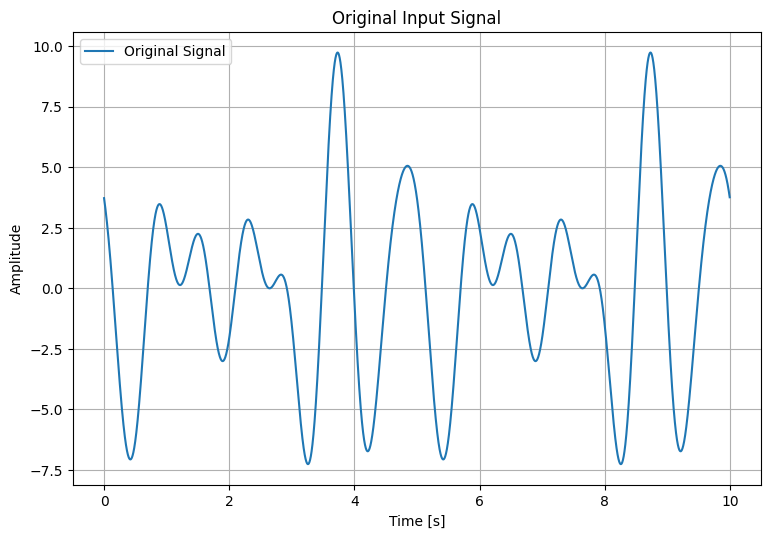
\includegraphics[width=\textwidth]{Figures/MultiFrequency/1_Input_Signal.png}
        \caption{Signal}
        \label{fig:mf_binmatch_input}
    \end{subfigure}
    \hfill
    \begin{subfigure}[b]{0.45\textwidth}
        \centering
        
\includegraphics[width=\textwidth]{Figures/MultiFrequency/1_Spectrum.png}
        \caption{Amplitude spectrum}
        \label{fig:mf_binmatch_spectrum}
    \end{subfigure}
    \caption{Multi-frequency bin-matched case: input signal and corresponding FFT spectrum with zero error across all components.}
    \label{fig:mf_binmatch}
\end{figure}

As shown in Table~\ref{tab:mf_binmatch} and Figure~\ref{fig:mf_binmatch}, all five frequency
components are extracted with zero error. This confirms that when all signal frequencies fall
on frequency bins, the FFT produces accurate results regardless of the number of frequency
components present.

% ------------------------------------------------------------
\subsection{Bin Match with Noise}
% ------------------------------------------------------------

The same multi-frequency signal is used here, with the addition of white noise at an amplitude
of 0.2. The aim is to assess whether the noise effect observed in the single-frequency case
persists under multi-frequency conditions.

\begin{table}[htbp]
\centering
\caption{FFT amplitude detection results for a multi-frequency bin-matched signal with added white noise.}
\label{tab:mf_binmatch_noise}
\begin{tabular}{|c|c|c|c|}
\hline
\textbf{Input Frequency (Hz)} & \textbf{Input Amplitude} & \textbf{FFT Amplitude} & \textbf{Error (\%)} \\
\hline
0.40  & 1.0 & 1.000 & 0.04 \\
\hline
0.80  & 4.0 & 4.000 & 0.15 \\
\hline
1.00  & 3.0 & 3.000 & 0.15 \\
\hline
1.20  & 1.0 & 1.000 & 0.09 \\
\hline
1.40  & 2.0 & 2.000 & 0.07 \\
\hline
\multicolumn{3}{|r|}{\textbf{Overall Error}} & \textbf{0.12\%} \\
\hline
\end{tabular}
\end{table}

\begin{figure}[htbp]
    \centering
    \begin{subfigure}[b]{0.45\textwidth}
        \centering
        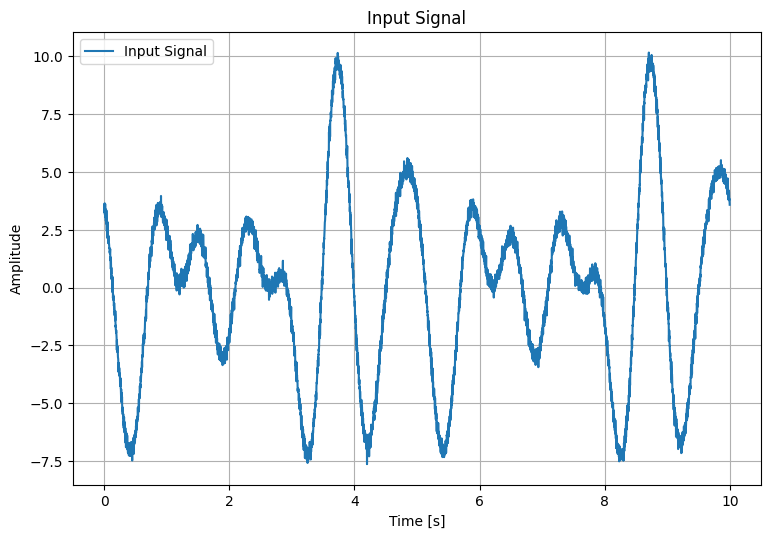
\includegraphics[width=\textwidth]{Figures/MultiFrequency/2_Input_Signal.png}        
        \caption{Signal}
        \label{fig:mf_noise_input}
    \end{subfigure}
    \hfill
    \begin{subfigure}[b]{0.45\textwidth}
        \centering
        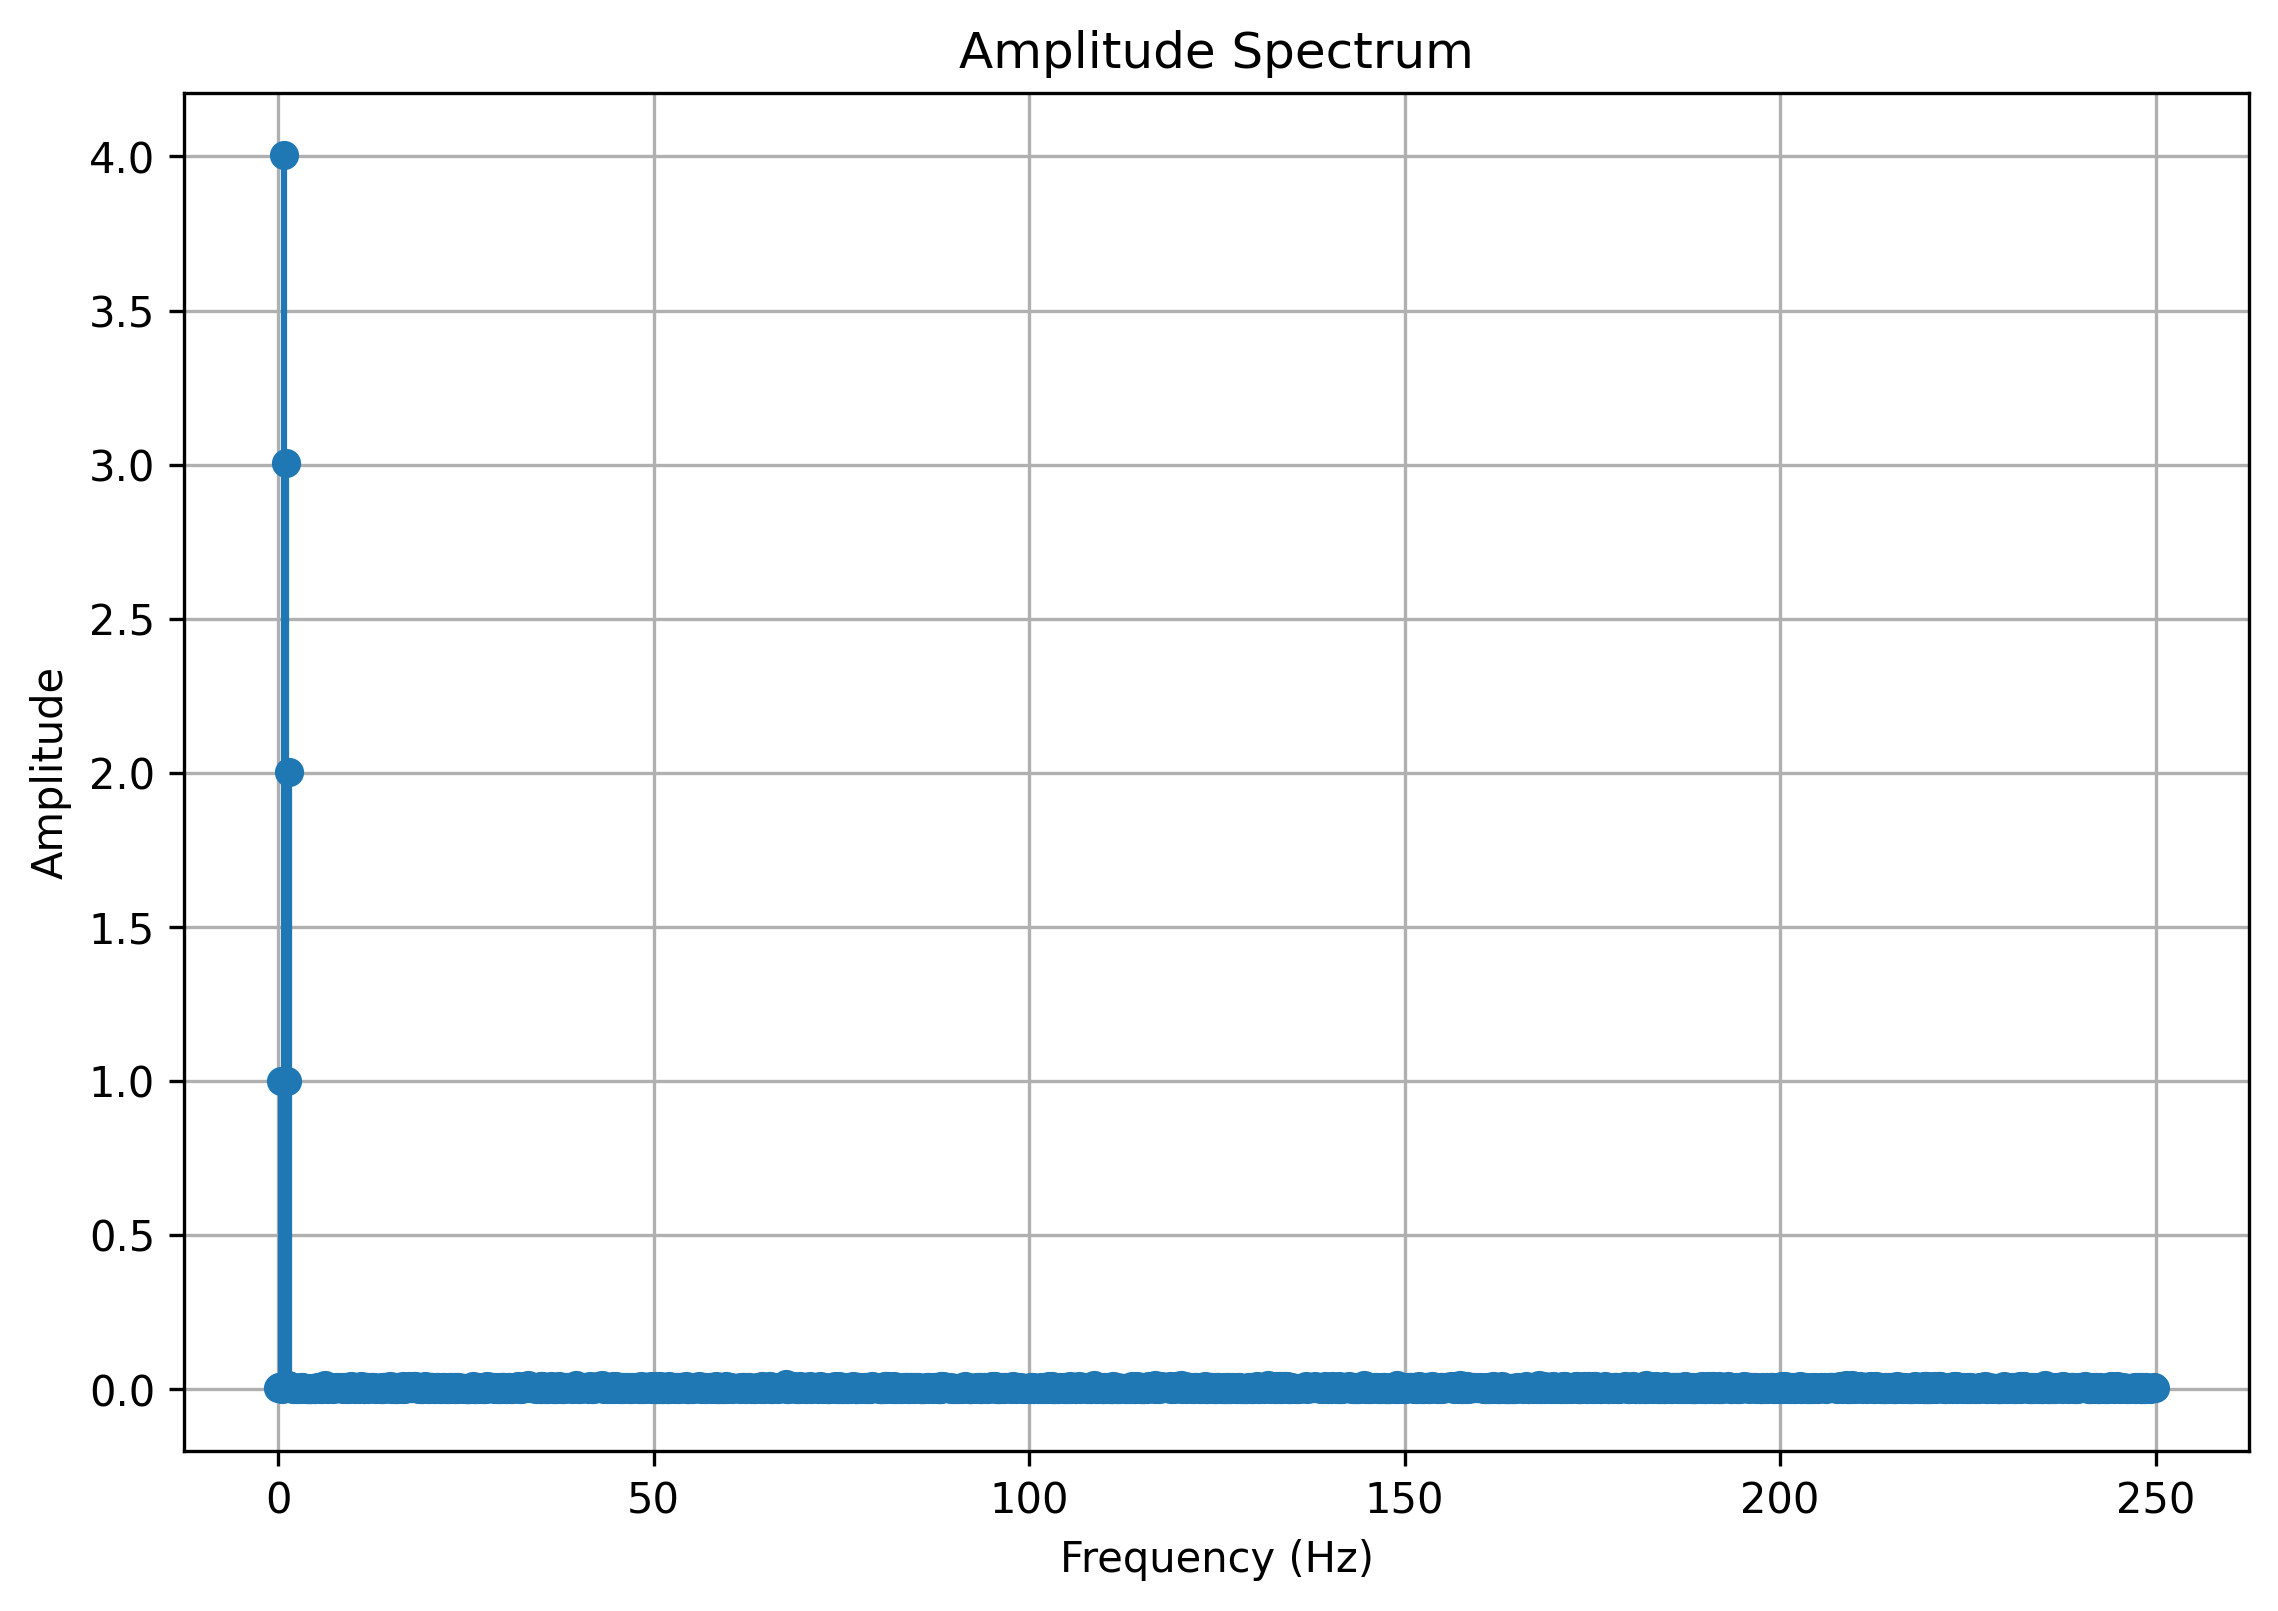
\includegraphics[width=\textwidth]{Figures/MultiFrequency/2_Spectrum.png}
        \caption{Amplitude spectrum}
        \label{fig:mf_noise_spectrum}
    \end{subfigure}
    \caption{Multi-frequency bin-matched case with added white noise: input signal and corresponding FFT spectrum.}
    \label{fig:mf_noise}
\end{figure}

As shown in Table~\ref{tab:mf_binmatch_noise} and Figure~\ref{fig:mf_noise}, the introduction
of white noise produces small errors across all frequency components. This result is consistent
with the single-frequency case with noise, where the errors remain small relative to those caused by spectral
leakage. White noise produces uniform amplitude perturbations across the entire frequency spectrum.
Consequently, each amplitude component experiences the same level of disturbance regardless of how many signals 
are superposed. Hence, the result is consistent in both cases.

% ------------------------------------------------------------
\subsection{One Component Non-Bin-Matched}
% ------------------------------------------------------------

In this case, the effect of a single frequency (within the multi-frequency signal) not falling on a frequency bin is
investigated, specifically to check whether the
resulting error is isolated to the non-matching frequency or propagates to
neighbouring frequency components as well.\\

To investigate this, a multi-frequency signal identical to the previous case is used, with an
additional component at 1.05~Hz introduced. Since the frequency bins are located at 1.0~Hz
and 1.1~Hz, this frequency falls exactly midway between two adjacent bins, making it a
worst-case spectral leakage scenario.

\begin{table}[htbp]
\centering
\caption{FFT amplitude detection results for a multi-frequency signal with one non-bin-matched component at 1.05~Hz.}
\label{tab:mf_nonbinmatch}
\begin{tabular}{|c|c|c|c|}
\hline
\textbf{Input Frequency (Hz)} & \textbf{Input Amplitude} & \textbf{FFT Amplitude} & \textbf{Error (\%)} \\
\hline
0.40  & 1.0 & 1.0095 &  0.95 \\
\hline
0.80  & 4.0 & 3.8793 &  3.02 \\
\hline
1.00  & 3.0 & 2.4999 & 16.67 \\
\hline
1.05  & 1.0 & 0.9654 &  3.45 \\
\hline
1.10  & 1.0 & 0.2145 & 78.55 \\
\hline
1.40  & 2.0 & 2.0152 &  0.76 \\
\hline
\multicolumn{3}{|r|}{\textbf{Overall Error}} & \textbf{17.23\%} \\
\hline
\end{tabular}
\end{table}

\begin{figure}[htbp]
    \centering
    \begin{subfigure}[b]{0.45\textwidth}
        \centering   
        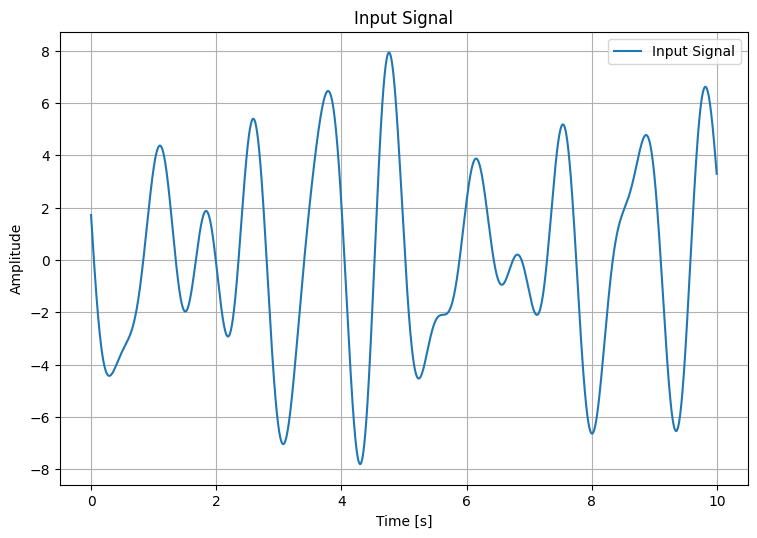
\includegraphics[width=\textwidth]{Figures/MultiFrequency/3_Input_Signal.png}
        \caption{Signal}
        \label{fig:mf_nonbinmatch_input}
    \end{subfigure}
    \hfill
    \begin{subfigure}[b]{0.45\textwidth}
        \centering
        
\includegraphics[width=\textwidth]{Figures/MultiFrequency/3_Spectrum.png}
        \caption{Amplitude spectrum}
        \label{fig:mf_nonbinmatch_spectrum}
    \end{subfigure}
    \caption{Multi-frequency case with one non-bin-matched component at 1.05~Hz: input signal and FFT 
spectrum illustrating leakage into neighbouring bins.}
    \label{fig:mf_nonbinmatch}
\end{figure}

As shown in Table~\ref{tab:mf_nonbinmatch} and Figure~\ref{fig:mf_nonbinmatch}, spectral
leakage from the 1.05~Hz component does not remain isolated to that frequency alone. It also
corrupts the amplitudes of neighbouring frequency components, particularly 1.00~Hz and
1.10~Hz, which exhibit errors of 16.67\% and 78.55\% respectively.\\

A key observation is that the magnitude of this leakage-induced error decreases with
increasing spectral distance from the non-bin-matched frequency. This spatial decay of leakage
is also visible in the FFT spectrum, where the spurious disturbance diminishes progressively
at frequencies further from 1.05~Hz. This behaviour denotes the importance of ensuring
all frequency components in a multi-frequency signal fall on frequency bins.

% ============================================================
\section{Discussions}
% ============================================================
The signal analysis conducted in this chapter provide important insights into the Fast Fourier Transform (FFT) and its limitations
when applied to the extraction of signals. The study showed that when a signal frequency coincides exactly with an FFT frequency bin, the amplitude is identified without significant error, 
both for single-frequency and multi-frequency signals. However, when a frequency component does not fall on a bin (non-bin-matched case), spectral leakage 
introduces significant amplitude errors. In the single-frequency case, these errors can exceed 20\%, depending on the relative position of the signal 
within the bin interval. In multi-frequency signals, spectral leakage from a single non-bin-matched component 
propagates to neighbouring frequencies, causing errors in their extracted amplitudes as well as to overall errors.
White noise had a comparatively minor influence on amplitude extraction accuracy when frequencies are properly 
aligned with frequency bins, confirming that spectral leakage is the dominant source of error in FFT-based multi-frequency 
analysis. \\

The frequency resolution, determined by the length of the data record (\(T = N/f_s\)), plays an important role in reducing spectral 
leakage. If the length of the data record is increased, the possibility that signal frequencies fall close to a frequency bin in 
relative terms increases, thereby reducing leakage-induced errors. However, the sensitivity of the error to the exact relative 
position within a bin also increases with finer resolution. Hence, careful selection of simulation time and excitation 
frequencies is needed. \\

These results illustrate the importance of frequency selection in the multi-frequency method for flutter derivative identification. 
When performing the multi-frequency simulations, prescribed motion frequencies should be chosen such that they coincide with 
FFT frequency bins for the chosen data length (total simulation time steps) and sampling frequency (\(1/\Delta t\)). \\

\end{document}